\documentclass[a4paper]{article}

\usepackage{amsmath}
\usepackage{hyperref}
\usepackage{graphicx}

% Document properties
\setlength{\parindent}{0pt}
\setlength{\parskip}{1ex plus 0.5ex minus 0.2ex}
\date{\today}
\title{Using local binary patterns to read license plates in photographs}
\author{
    Gijs van der Voort\\
    Richard Torenvliet\\
    Jayke Meijer\\
    Tadde\"us Kroes\\
    Fabi\"en Tesselaar
}

% Front page / toc
\begin{document}
\maketitle
\thispagestyle{empty}
\newpage
\tableofcontents
\newpage


\section{Problem description}

License plates are used for uniquely identifying motorized vehicles and are made
to be read by humans from great distances and in all kinds of weather
conditions.

Reading license plates with a computer is much more difficult. Our dataset
contains photographs of license plates from various angles and distances. This
means that not only do we have to implement a method to read the actual
characters, but given the location of the license plate and each individual
character, we must make sure we transform each character to a standard form.
This has to be done or else the local binary patterns will never match!

Determining what character we are looking at will be done by using Local Binary
Patterns. The main goal of our research is finding out how effective LBP's are
in classifying characters on a license plate.


\section{The process}

The process with which we extract license places from photographs consists of
multiple steps listed below. All these steps will be explained in detail further
on in this report.

\begin{enumerate}
    \item Extract character images from a license plate photograph using the
          location points in the XML files from our dataset.
    \item Reduce the noise in a character image using a Gaussian filter.
    \item Transforming a character image to a normal form.
    \item Create a LBP histogram vector for a character image.
    \item Match the a feature vector with a learning set using a SVM.
    \item Verify the match given by the SVM against our dataset.
\end{enumerate}


\section{The dataset}

The dataset consists of photographs of license plates from various angles and
distances. The photographs are all 8-bit gray-scale JPEG images. With every
photograph there is a .info file. These files, consisting of XML data, contain
information about the photographed license plate like the country, information
about the image, the location of the license plate and the location of the
characters in  the license plate.


\section{Implementation}


\subsection{Used programming language}

Although the actual purpose of this research is to see if LBP is capable of
recognizing license plate characters. We know that LBP is a fast algorithm thus
an advantage had to be its speed compared with other license plate recognition
implementations. The uncertainty of whether LBP's could get some results made us
pick Python.

Python is a very flexible programming language: there are a lot of existing
modules and frameworks most of which are made in C, the higher order of the
language makes programming applications quick and because it is fairly easy to
transform a python module to a C based module, our system could be easily
converted to a faster C implementation if our results are positive.


\subsection{Character extraction}


\subsubsection{Reading the INFO file}

The XML reader will return a 'license plate' object when given an XML file. The
license plate holds a list of, up to six, NormalizedImage characters and from
which country the plate is from. The reader is currently assuming the XML file
and image name are corresponding. Since this was the case for the given dataset.
This can easily be adjusted if required.

To parse the XML file, the minidom module is used. So the XML file can be
treated as a tree, where one can search for certain nodes. In each XML file it
is possible that multiple versions exist, so the first thing the reader will do
is retrieve the current and most up-to-date version of the plate. The reader
will only get results from this version.

Now we are only interested in the individual characters so we can skip the
location of the entire license plate. Each character has a single character
value, indicating what someone thought what the letter or digit was and four
coordinates to create a bounding box. To make things not to complicated a
Character class and Point class are used. They act pretty much as associative
lists, but it gives extra freedom on using the data. If less then four points
have been set the character will not be saved.

When four points have been gathered the data from the actual image is being
requested. For each corner a small margin is added (around 3 pixels) so that no
features will be lost and minimum amounts of new features will be introduced by
noise in the margin.

In the next section you can read more about the perspective transformation that
is being done. After the transformation the character can be saved: Converted to
gray-scale, but nothing further. This was used to create a learning set. If it
does not need to be saved as an actual image it will be converted to a
NormalizedImage. When these actions have been completed for each character the
license plate is usable in the rest of the code.


\subsubsection{Perspective transformation}

Once we retrieved the corner points of the character, we feed those to a module
that extracts the (warped) character from the original image, and creates a new
image where the character is cut out, and is transformed to a rectangle.



\subsection{Noise reduction}

Small amounts of noise will probably be suppressed by usage of a Gaussian
filter. A real problem occurs in very dirty license plates, where branches and
dirt over a letter could radically change the local binary pattern. A question
we can ask ourselves here, is whether we want to concentrate ourselves on these
exceptional cases. By law, license plates have to be readable. However, the
provided dataset showed that this does not means they always are.


\subsubsection{Camera noise and small amounts of dirt}

The dirt on the license plate can be of different sizes. We can reduce the
smaller amounts of dirt in the same way as we reduce normal noise, by applying a
Gaussian blur to the image. This is the next step in our program.

The Gaussian filter we use comes from the \texttt{scipy.ndimage} module. We use
this function instead of our own function, because the standard functions are
most likely more optimized then our own implementation, and speed is an
important factor in this application.


\subsubsection{Larger amounts of dirt}

Larger amounts of dirt are not going to be resolved by using a Gaussian filter.
We rely on one of the characteristics of the Local Binary Pattern, only looking
at the difference between two pixels, to take care of these problems.\\ Because
there will probably always be a difference between the characters and the dirt,
and the fact that the characters are very black, the shape of the characters
will still be conserved in the LBP, even if there is dirt surrounding the
character.


\subsection{Building a feature vector}


\subsubsection{Creating LBP's}

The LBP algorithm that we implemented is a square variant of LBP, the same that
is introduced by Ojala et al (1994). Wikipedia presents a different form where
the pattern is circular.

\begin{itemize}

\item Determine the size of the square where the local patterns are being
registered. For explanation purposes let the square be 3 x 3.

\item The gray-scale value of the middle pixel is used as threshold. Every value
of the pixel around the middle pixel is evaluated. If it's value is greater than
the threshold it will be become a one else a zero.

\begin{figure}[h!]
\center
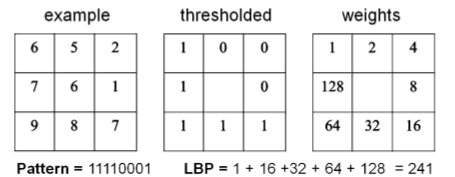
\includegraphics[scale=0.5]{lbp.png}
\caption{LBP 3 x 3 (Pietik\"ainen, Hadid, Zhao \& Ahonen (2011))}
\end{figure}

Notice that the pattern will be come of the form 01001110. This is done when a
the value of the evaluated pixel is greater than the threshold, shift the bit by
the n(with i=i$_{th}$ pixel evaluated, starting with $i=0$).

This results in a mathematical expression:

Let I($x_i, y_i$) an Image with gray-scale values and $g_n$ the gray-scale value
of the pixel $(x_i, y_i)$. Also let $s(g_i, g_c)$ (see below) with $g_c$ =
gray-scale value of the center pixel and $g_i$ the gray-scale value of the pixel
to be evaluated.

$$
  s(g_i, g_c) = \left\{
  \begin{array}{l l}
    1 & \quad \text{if $g_i$ $\geq$ $g_c$}\\
    0 & \quad \text{if $g_i$ $<$ $g_c$}\\
  \end{array} \right.
$$

$$LBP_{n, g_c = (x_c, y_c)} = \sum\limits_{i=0}^{n-1} s(g_i, g_c)^{2i} $$

The outcome of this operations will be a binary pattern.

\item Given this pattern, the next step is to divide the pattern in cells. The
amount of cells depends on the quality of the result, so trial and error is in
order. Starting with dividing the pattern in to cells of size 16.

\item Compute a histogram for each cell.

\begin{figure}[h!]
\center
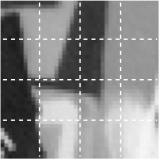
\includegraphics[scale=0.7]{cells.png}
\caption{Divide in cells(Pietik\"ainen et all (2011))}
\end{figure}

\item Consider every histogram as a vector element and concatenate these. The
result is a feature vector of the image.

\item Feed these vectors to a support vector machine. This will 'learn' which
vector indicates what vector is which character.

\end{itemize}

\begin{figure}[h!]
\center
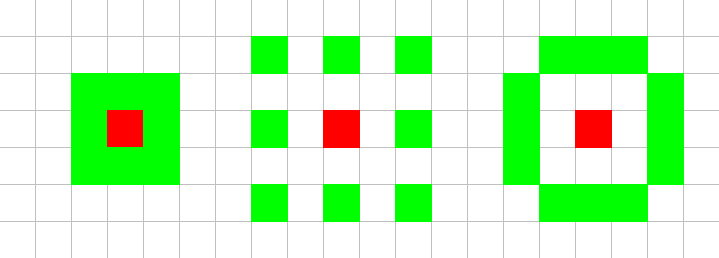
\includegraphics[scale=0.5]{neighbourhoods.png}
\caption{Tested neighborhoods}
\end{figure}

We have tried the neighborhoods as showed in figure 3. We chose these
neighborhoods to prevent having to use interpolation, which would add a
computational step, thus making the code execute slower. In the next section we
will describe what the best neighborhood was.

Take an example where the full square can be evaluated, there are cases where
the neighbors are out of bounds. The first to be checked is the pixel in the
left bottom corner in the square 3 x 3, with coordinate $(x - 1, y - 1)$ with
$g_c$ as center pixel that has coordinates $(x, y)$. If the gray-scale value of
the neighbor in the left corner is greater than the gray-scale value of the
center pixel than return true. Bit-shift the first bit with 7. The outcome is
now 1000000. The second neighbor will be bit-shifted with 6, and so on. Until we
are at 0. The result is a binary pattern of the local point just evaluated. Now
only the edge pixels are a problem, but a simple check if the location of the
neighbor is still in the image can resolve this. We simply return false if it
is.


\subsubsection{Creating histograms and the feature vector}

After all the Local Binary Patterns are created for every pixel. This pattern is
divided in to cells. The feature vector is the vector of concatenated
histograms. These histograms are created for cells. These cells are created by
dividing the \textbf{pattern} in to cells and create a histogram of that. So
multiple cells are related to one histogram. All the histograms are concatenated
and fed to the SVM that will be discussed in the next section, Classification.
We did however find out that the use of several cells was not increasing our
performance, so we only have one histogram to feed to the SVM.


\subsection{Matching the database}

Given the LBP of a character, a Support Vector Machine can be used to classify
the character to a character in a learning set. The SVM uses a concatenation of
each cell in an image as a feature vector (in the case we check the entire image
no concatenation has to be done of course. The SVM can be trained with a subset
of the given dataset called the Learning set. Once trained, the entire
classifier can be saved as a Pickle object\footnote{See
\url{http://docs.python.org/library/pickle.html}} for later usage.


\section{Determining optimal parameters}

Now that we have a functioning system, we need to tune it to work properly for
license plates. This means we need to find the parameters. Throughout the
program we have a number of parameters for which no standard choice is
available. These parameters are:

\begin{tabular}{l|l}
  Parameter       & Description\\
  \hline
  $\sigma$        & The size of the Gaussian blur.\\
  \emph{cell size}  & The size of a cell for which a histogram of LBP's
                        will be generated.\\
  \emph{Neighborhood}& The neighborhood to use for creating the LBP.\\
  $\gamma$      & Parameter for the Radial kernel used in the SVM.\\
  $c$         & The soft margin of the SVM. Allows how much training
              errors are accepted.\\
\end{tabular}

For each of these parameters, we will describe how we searched for a good value,
and what value we decided on.


\subsection{Parameter $\sigma$}

The first parameter to decide on, is the $\sigma$ used in the Gaussian blur. To
find this parameter, we tested a few values, by checking visually what value
removed most noise out of the image, while keeping the edges sharp enough to
work with. It turned out the best value is $\sigma = 0.5$.


\subsection{Parameter \emph{cell size}}

The cell size of the Local Binary Patterns determines over what region a
histogram is made. The trade-off here is that a bigger cell size makes the
classification less affected by relative movement of a character compared to
those in the learning set, since the important structure will be more likely to
remain in the same cell. However, if the cell size is too big, there will not be
enough cells to properly describe the different areas of the character, and the
feature vectors will not have enough elements.

In order to find this parameter, we used a trial-and-error technique on a few
cell sizes. During this testing, we discovered that a lot better score was
reached when we take the histogram over the entire image, so with a single cell.
Therefore, we decided to work without cells.

The reason that using one cell works best is probably because the size of a
single character on a license plate in the provided dataset is very small. That
means that when dividing it into cells, these cells become simply too small to
have a really representative histogram. Therefore, the concatenated histograms
are then a list of only very small numbers, which are not significant enough to
allow for reliable classification.


\subsection{Parameter \emph{Neighborhood}}

The neighborhood to use can only be determined through testing. We did a test
with each of these neighborhoods, and we found that the best results were
reached with the following neighborhood, which we will call the ()-neighborhood.


\subsection{Parameter $\gamma$ \& $c$}

The parameters $\gamma$ and $c$ are used for the SVM. $c$ is a standard
parameter for each type of SVM, called the 'soft margin'. This indicates how
exact each element in the learning set should be taken. A large soft margin
means that an element in the learning set that accidentally has a completely
different feature vector than expected, due to noise for example, is not taken
into account. If the soft margin is very small, then almost all vectors will be
taken into account, unless they differ extreme amounts.

$\gamma$ is a variable that determines the size of the radial kernel, and as
such determines how steep the difference between two classes can be.

Since these parameters both influence the SVM, we need to find the best
combination of values. To do this, we perform a so-called grid-search. A grid-
search takes exponentially growing sequences for each parameter, and checks for
each combination of values what the score is. The combination with the highest
score is then used as our parameters, and the entire SVM will be trained using
those parameters.

We found that the best values for these parameters are $c = ?$ and $\gamma = ?$.


\section{Results}


\subsection{Speed}

Recognizing license plates is something that has to be done fast, since there
can be a lot of cars passing a camera in a short time, especially on a highway.
Therefore, we measured how well our program performed in terms of speed. We
measure the time used to classify a license plate, not the training of the
dataset, since that can be done off-line, and speed is not a primary necessity
there.

The speed of a classification turned out to be ???.


\subsection{Accuracy}

Of course, it is vital that the recognition of a license plate is correct,
almost correct is not good enough here. Therefore, we have to get the highest
accuracy score we possibly can.

According to Wikipedia \footnote{
\url{http://en.wikipedia.org/wiki/Automatic_number_plate_recognition}},
commercial license plate recognition software score about $90\%$ to $94\%$,
under optimal conditions and with modern equipment.

Our program scores an average of ???.


\section{Conclusion}

It turns out that using Local Binary Patterns is a promising technique for
License Plate Recognition. It seems to be relatively insensitive by dirty
license plates and different fonts on these plates.

The performance speed wise is ???


\section{Reflection}


\subsection{Dataset}

The first problem was that the dataset contains a lot of license plates which
are problematic to read, due to excessive amounts of dirt on them. Of course,
this is something you would encounter in the real situation, but it made it hard
for us to see whether there was a coding error or just a bad example.

Another problem was that there were license plates of several countries in the
dataset. Each of these countries has it own font, which also makes it hard to
identify these plates, unless there are a lot of these plates in the learning
set.

A problem that is more elemental is that some of the characters in the dataset
are not properly classified. This is of course very problematic, both for
training the SVM as for checking the performance. This meant we had to check
each character whether its description was correct.


\subsection{SVM}

We also had trouble with the SVM for Python. The standard Python SVM, libsvm,
had a poor documentation. There was no explanation what so ever on which
parameter had to be what. This made it a lot harder for us to see what went
wrong in the program.


\subsection{Workload distribution}

The first two weeks were team based. Basically the LBP algorithm could be
implemented in the first hour, while some talked and someone did the typing.
Some additional 'basics' where created in similar fashion. This ensured that
every team member was up-to-date and could start figuring out which part of the
implementation was most suited to be done by one individually or in a pair.

Gijs created the basic classes we could use and helped the rest everyone by
keeping track of what required to be finished and whom was working on what.
Tadde\"us and Jayke were mostly working on the SVM and all kinds of tests
whether the histograms were matching and alike. Fabi\"en created the functions
to read and parse the given xml files with information about the license plates.
Upon completion all kinds of learning and data sets could be created.

%Richard je moet even toevoegen wat je hebt gedaan :P:P maar miss is dit hele
%ding wel overbodig Ik dacht dat Rein het zei tijdens gesprek van ik wil weten
%hoe het ging enzo.

Sometimes one cannot hear the alarm bell and wake up properly. This however was
not a big problem as no one was afraid of staying at Science Park a bit longer
to help out. Further communication usually went through e-mails and replies were
instantaneous! A crew to remember.


\end{document}
